% Generated by Sphinx.
\def\sphinxdocclass{report}
\documentclass[letterpaper,10pt,english]{sphinxmanual}
\usepackage[utf8]{inputenc}
\DeclareUnicodeCharacter{00A0}{\nobreakspace}
\usepackage{cmap}
\usepackage[T1]{fontenc}
\usepackage{babel}
\usepackage{times}
\usepackage[Bjarne]{fncychap}
\usepackage{longtable}
\usepackage{sphinx}
\usepackage{multirow}


\title{matchApp Documentation}
\date{June 22, 2016}
\release{2}
\author{Grupo5}
\newcommand{\sphinxlogo}{}
\renewcommand{\releasename}{Release}
\makeindex

\makeatletter
\def\PYG@reset{\let\PYG@it=\relax \let\PYG@bf=\relax%
    \let\PYG@ul=\relax \let\PYG@tc=\relax%
    \let\PYG@bc=\relax \let\PYG@ff=\relax}
\def\PYG@tok#1{\csname PYG@tok@#1\endcsname}
\def\PYG@toks#1+{\ifx\relax#1\empty\else%
    \PYG@tok{#1}\expandafter\PYG@toks\fi}
\def\PYG@do#1{\PYG@bc{\PYG@tc{\PYG@ul{%
    \PYG@it{\PYG@bf{\PYG@ff{#1}}}}}}}
\def\PYG#1#2{\PYG@reset\PYG@toks#1+\relax+\PYG@do{#2}}

\expandafter\def\csname PYG@tok@gd\endcsname{\def\PYG@tc##1{\textcolor[rgb]{0.63,0.00,0.00}{##1}}}
\expandafter\def\csname PYG@tok@gu\endcsname{\let\PYG@bf=\textbf\def\PYG@tc##1{\textcolor[rgb]{0.50,0.00,0.50}{##1}}}
\expandafter\def\csname PYG@tok@gt\endcsname{\def\PYG@tc##1{\textcolor[rgb]{0.00,0.27,0.87}{##1}}}
\expandafter\def\csname PYG@tok@gs\endcsname{\let\PYG@bf=\textbf}
\expandafter\def\csname PYG@tok@gr\endcsname{\def\PYG@tc##1{\textcolor[rgb]{1.00,0.00,0.00}{##1}}}
\expandafter\def\csname PYG@tok@cm\endcsname{\let\PYG@it=\textit\def\PYG@tc##1{\textcolor[rgb]{0.25,0.50,0.56}{##1}}}
\expandafter\def\csname PYG@tok@vg\endcsname{\def\PYG@tc##1{\textcolor[rgb]{0.73,0.38,0.84}{##1}}}
\expandafter\def\csname PYG@tok@m\endcsname{\def\PYG@tc##1{\textcolor[rgb]{0.13,0.50,0.31}{##1}}}
\expandafter\def\csname PYG@tok@mh\endcsname{\def\PYG@tc##1{\textcolor[rgb]{0.13,0.50,0.31}{##1}}}
\expandafter\def\csname PYG@tok@cs\endcsname{\def\PYG@tc##1{\textcolor[rgb]{0.25,0.50,0.56}{##1}}\def\PYG@bc##1{\setlength{\fboxsep}{0pt}\colorbox[rgb]{1.00,0.94,0.94}{\strut ##1}}}
\expandafter\def\csname PYG@tok@ge\endcsname{\let\PYG@it=\textit}
\expandafter\def\csname PYG@tok@vc\endcsname{\def\PYG@tc##1{\textcolor[rgb]{0.73,0.38,0.84}{##1}}}
\expandafter\def\csname PYG@tok@il\endcsname{\def\PYG@tc##1{\textcolor[rgb]{0.13,0.50,0.31}{##1}}}
\expandafter\def\csname PYG@tok@go\endcsname{\def\PYG@tc##1{\textcolor[rgb]{0.20,0.20,0.20}{##1}}}
\expandafter\def\csname PYG@tok@cp\endcsname{\def\PYG@tc##1{\textcolor[rgb]{0.00,0.44,0.13}{##1}}}
\expandafter\def\csname PYG@tok@gi\endcsname{\def\PYG@tc##1{\textcolor[rgb]{0.00,0.63,0.00}{##1}}}
\expandafter\def\csname PYG@tok@gh\endcsname{\let\PYG@bf=\textbf\def\PYG@tc##1{\textcolor[rgb]{0.00,0.00,0.50}{##1}}}
\expandafter\def\csname PYG@tok@ni\endcsname{\let\PYG@bf=\textbf\def\PYG@tc##1{\textcolor[rgb]{0.84,0.33,0.22}{##1}}}
\expandafter\def\csname PYG@tok@nl\endcsname{\let\PYG@bf=\textbf\def\PYG@tc##1{\textcolor[rgb]{0.00,0.13,0.44}{##1}}}
\expandafter\def\csname PYG@tok@nn\endcsname{\let\PYG@bf=\textbf\def\PYG@tc##1{\textcolor[rgb]{0.05,0.52,0.71}{##1}}}
\expandafter\def\csname PYG@tok@no\endcsname{\def\PYG@tc##1{\textcolor[rgb]{0.38,0.68,0.84}{##1}}}
\expandafter\def\csname PYG@tok@na\endcsname{\def\PYG@tc##1{\textcolor[rgb]{0.25,0.44,0.63}{##1}}}
\expandafter\def\csname PYG@tok@nb\endcsname{\def\PYG@tc##1{\textcolor[rgb]{0.00,0.44,0.13}{##1}}}
\expandafter\def\csname PYG@tok@nc\endcsname{\let\PYG@bf=\textbf\def\PYG@tc##1{\textcolor[rgb]{0.05,0.52,0.71}{##1}}}
\expandafter\def\csname PYG@tok@nd\endcsname{\let\PYG@bf=\textbf\def\PYG@tc##1{\textcolor[rgb]{0.33,0.33,0.33}{##1}}}
\expandafter\def\csname PYG@tok@ne\endcsname{\def\PYG@tc##1{\textcolor[rgb]{0.00,0.44,0.13}{##1}}}
\expandafter\def\csname PYG@tok@nf\endcsname{\def\PYG@tc##1{\textcolor[rgb]{0.02,0.16,0.49}{##1}}}
\expandafter\def\csname PYG@tok@si\endcsname{\let\PYG@it=\textit\def\PYG@tc##1{\textcolor[rgb]{0.44,0.63,0.82}{##1}}}
\expandafter\def\csname PYG@tok@s2\endcsname{\def\PYG@tc##1{\textcolor[rgb]{0.25,0.44,0.63}{##1}}}
\expandafter\def\csname PYG@tok@vi\endcsname{\def\PYG@tc##1{\textcolor[rgb]{0.73,0.38,0.84}{##1}}}
\expandafter\def\csname PYG@tok@nt\endcsname{\let\PYG@bf=\textbf\def\PYG@tc##1{\textcolor[rgb]{0.02,0.16,0.45}{##1}}}
\expandafter\def\csname PYG@tok@nv\endcsname{\def\PYG@tc##1{\textcolor[rgb]{0.73,0.38,0.84}{##1}}}
\expandafter\def\csname PYG@tok@s1\endcsname{\def\PYG@tc##1{\textcolor[rgb]{0.25,0.44,0.63}{##1}}}
\expandafter\def\csname PYG@tok@gp\endcsname{\let\PYG@bf=\textbf\def\PYG@tc##1{\textcolor[rgb]{0.78,0.36,0.04}{##1}}}
\expandafter\def\csname PYG@tok@sh\endcsname{\def\PYG@tc##1{\textcolor[rgb]{0.25,0.44,0.63}{##1}}}
\expandafter\def\csname PYG@tok@ow\endcsname{\let\PYG@bf=\textbf\def\PYG@tc##1{\textcolor[rgb]{0.00,0.44,0.13}{##1}}}
\expandafter\def\csname PYG@tok@sx\endcsname{\def\PYG@tc##1{\textcolor[rgb]{0.78,0.36,0.04}{##1}}}
\expandafter\def\csname PYG@tok@bp\endcsname{\def\PYG@tc##1{\textcolor[rgb]{0.00,0.44,0.13}{##1}}}
\expandafter\def\csname PYG@tok@c1\endcsname{\let\PYG@it=\textit\def\PYG@tc##1{\textcolor[rgb]{0.25,0.50,0.56}{##1}}}
\expandafter\def\csname PYG@tok@kc\endcsname{\let\PYG@bf=\textbf\def\PYG@tc##1{\textcolor[rgb]{0.00,0.44,0.13}{##1}}}
\expandafter\def\csname PYG@tok@c\endcsname{\let\PYG@it=\textit\def\PYG@tc##1{\textcolor[rgb]{0.25,0.50,0.56}{##1}}}
\expandafter\def\csname PYG@tok@mf\endcsname{\def\PYG@tc##1{\textcolor[rgb]{0.13,0.50,0.31}{##1}}}
\expandafter\def\csname PYG@tok@err\endcsname{\def\PYG@bc##1{\setlength{\fboxsep}{0pt}\fcolorbox[rgb]{1.00,0.00,0.00}{1,1,1}{\strut ##1}}}
\expandafter\def\csname PYG@tok@mb\endcsname{\def\PYG@tc##1{\textcolor[rgb]{0.13,0.50,0.31}{##1}}}
\expandafter\def\csname PYG@tok@ss\endcsname{\def\PYG@tc##1{\textcolor[rgb]{0.32,0.47,0.09}{##1}}}
\expandafter\def\csname PYG@tok@sr\endcsname{\def\PYG@tc##1{\textcolor[rgb]{0.14,0.33,0.53}{##1}}}
\expandafter\def\csname PYG@tok@mo\endcsname{\def\PYG@tc##1{\textcolor[rgb]{0.13,0.50,0.31}{##1}}}
\expandafter\def\csname PYG@tok@kd\endcsname{\let\PYG@bf=\textbf\def\PYG@tc##1{\textcolor[rgb]{0.00,0.44,0.13}{##1}}}
\expandafter\def\csname PYG@tok@mi\endcsname{\def\PYG@tc##1{\textcolor[rgb]{0.13,0.50,0.31}{##1}}}
\expandafter\def\csname PYG@tok@kn\endcsname{\let\PYG@bf=\textbf\def\PYG@tc##1{\textcolor[rgb]{0.00,0.44,0.13}{##1}}}
\expandafter\def\csname PYG@tok@o\endcsname{\def\PYG@tc##1{\textcolor[rgb]{0.40,0.40,0.40}{##1}}}
\expandafter\def\csname PYG@tok@kr\endcsname{\let\PYG@bf=\textbf\def\PYG@tc##1{\textcolor[rgb]{0.00,0.44,0.13}{##1}}}
\expandafter\def\csname PYG@tok@s\endcsname{\def\PYG@tc##1{\textcolor[rgb]{0.25,0.44,0.63}{##1}}}
\expandafter\def\csname PYG@tok@kp\endcsname{\def\PYG@tc##1{\textcolor[rgb]{0.00,0.44,0.13}{##1}}}
\expandafter\def\csname PYG@tok@w\endcsname{\def\PYG@tc##1{\textcolor[rgb]{0.73,0.73,0.73}{##1}}}
\expandafter\def\csname PYG@tok@kt\endcsname{\def\PYG@tc##1{\textcolor[rgb]{0.56,0.13,0.00}{##1}}}
\expandafter\def\csname PYG@tok@sc\endcsname{\def\PYG@tc##1{\textcolor[rgb]{0.25,0.44,0.63}{##1}}}
\expandafter\def\csname PYG@tok@sb\endcsname{\def\PYG@tc##1{\textcolor[rgb]{0.25,0.44,0.63}{##1}}}
\expandafter\def\csname PYG@tok@k\endcsname{\let\PYG@bf=\textbf\def\PYG@tc##1{\textcolor[rgb]{0.00,0.44,0.13}{##1}}}
\expandafter\def\csname PYG@tok@se\endcsname{\let\PYG@bf=\textbf\def\PYG@tc##1{\textcolor[rgb]{0.25,0.44,0.63}{##1}}}
\expandafter\def\csname PYG@tok@sd\endcsname{\let\PYG@it=\textit\def\PYG@tc##1{\textcolor[rgb]{0.25,0.44,0.63}{##1}}}

\def\PYGZbs{\char`\\}
\def\PYGZus{\char`\_}
\def\PYGZob{\char`\{}
\def\PYGZcb{\char`\}}
\def\PYGZca{\char`\^}
\def\PYGZam{\char`\&}
\def\PYGZlt{\char`\<}
\def\PYGZgt{\char`\>}
\def\PYGZsh{\char`\#}
\def\PYGZpc{\char`\%}
\def\PYGZdl{\char`\$}
\def\PYGZhy{\char`\-}
\def\PYGZsq{\char`\'}
\def\PYGZdq{\char`\"}
\def\PYGZti{\char`\~}
% for compatibility with earlier versions
\def\PYGZat{@}
\def\PYGZlb{[}
\def\PYGZrb{]}
\makeatother

\renewcommand\PYGZsq{\textquotesingle}

\begin{document}

\maketitle
\tableofcontents
\phantomsection\label{index::doc}


Contenidos:


\chapter{Manual de Usuario}
\label{manuals:manual-de-usuario}\label{manuals::doc}\label{manuals:documentacion-de-matchapp}
\textbf{Grupo 10}

\textbf{Taller de Programación II}

\textbf{Ayudante: Christian Calonico}

\textbf{Integrantes:}

\begin{tabulary}{\linewidth}{|L|L|}
\hline
\textsf{\relax 
Apellido y Nombre
} & \textsf{\relax 
Padrón
}\\
\hline
Daye, Gisela Denise
 & 
87602
\\
\hline
Federico, Pablo
 & 
90280
\\
\hline
Farina, Federico
 & 
90177
\\
\hline
Vazquez, Nicolás
 & 
89172
\\
\hline\end{tabulary}



\section{Cliente}
\label{manuals:cliente}\begin{itemize}
\item {} 
Instalar apk en el telefono celular

\end{itemize}

\href{https://drive.google.com/open?id=0B96FtE1h2ukFNHdob042a3ZQU1k}{https://drive.google.com/open?id=0B96FtE1h2ukFNHdob042a3ZQU1k}
\begin{itemize}
\item {} 
Ejecutar el Application server en su pc seteando como ip de su Pc 192.168.1.33

\item {} 
Abrir aplicacion en el celular

\item {} 
Se encontrara con la pantalla de login

\end{itemize}

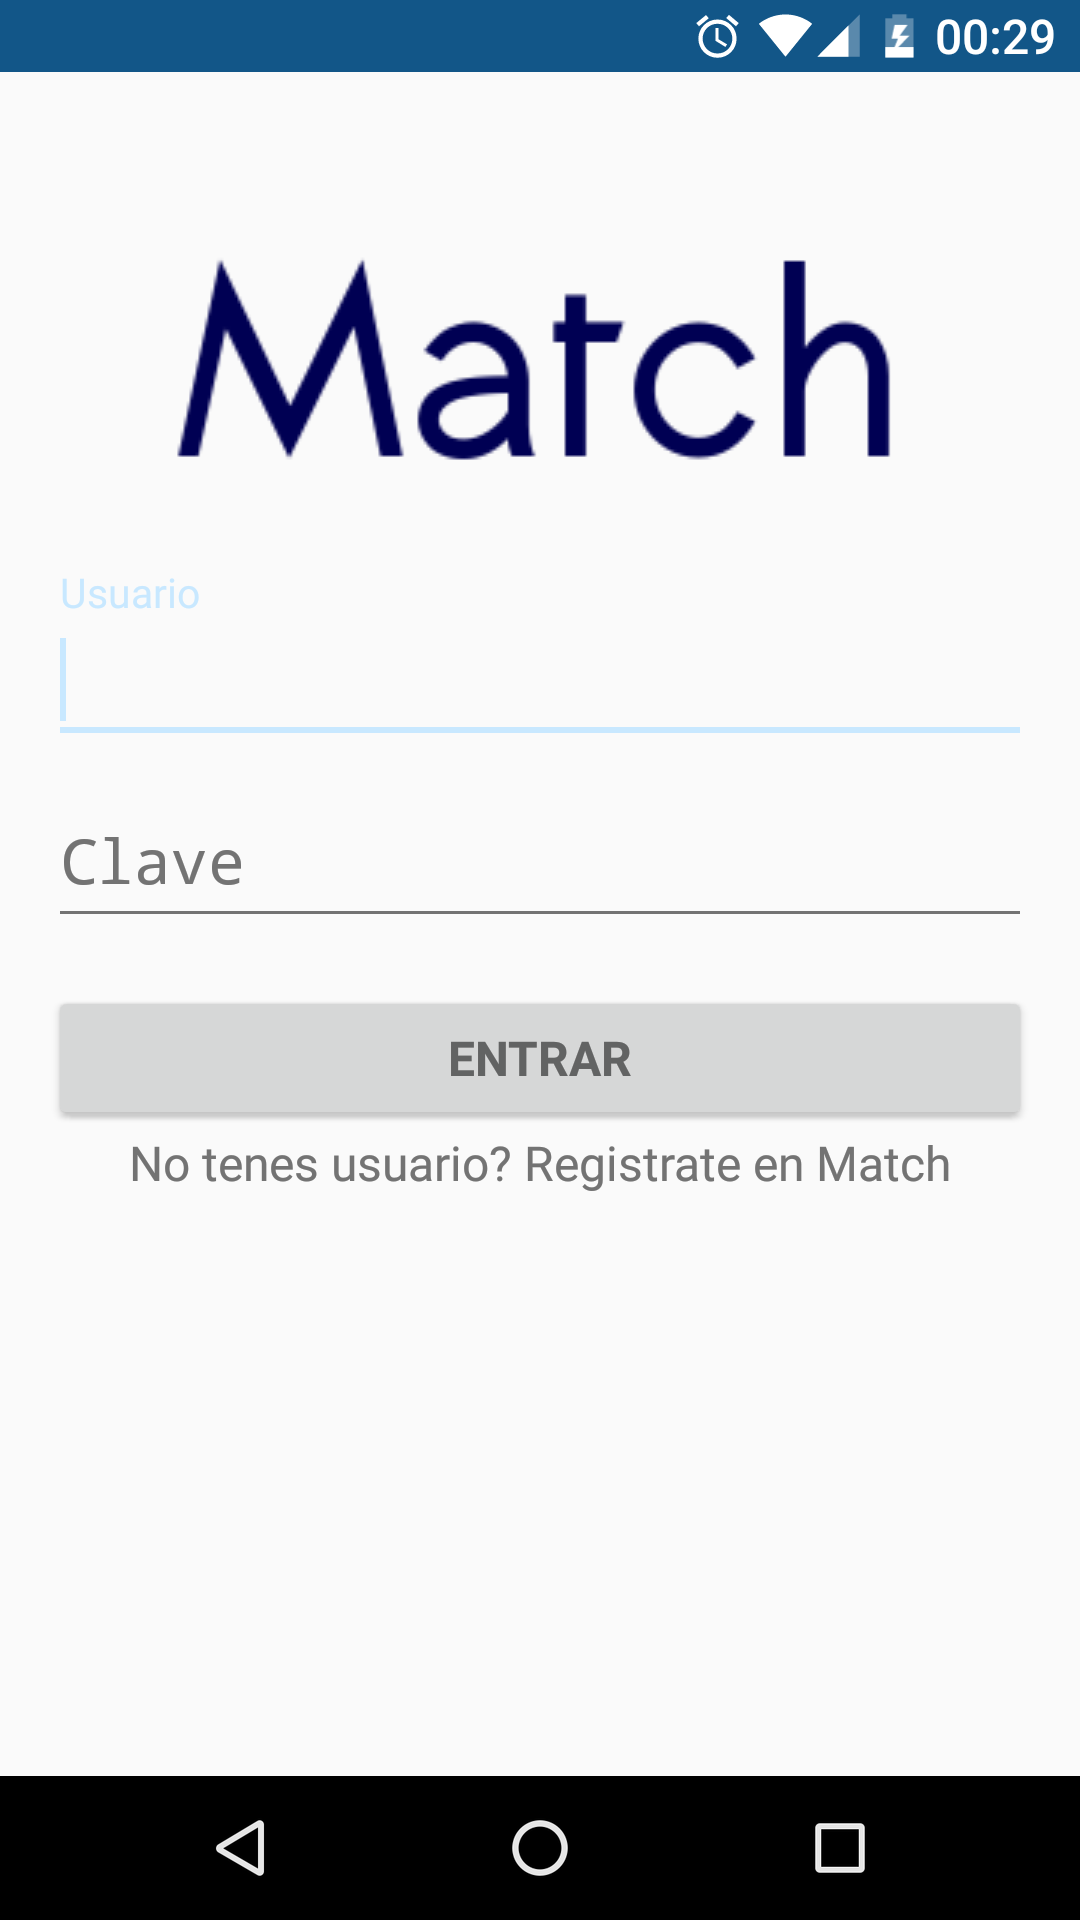
\includegraphics{login.png}
\begin{itemize}
\item {} 
Si ya posee un usuario registrado, ingrese los campos requeridos de usuario y clave y luego haga tap en el boton de entrar. Si los datos son los correctos se lo redireccionara a la pantalla de busqueda de matchs

\item {} 
Si los datos son incorrectos aparecera un mensaje de error y debera volver a intentar loguearse.

\end{itemize}

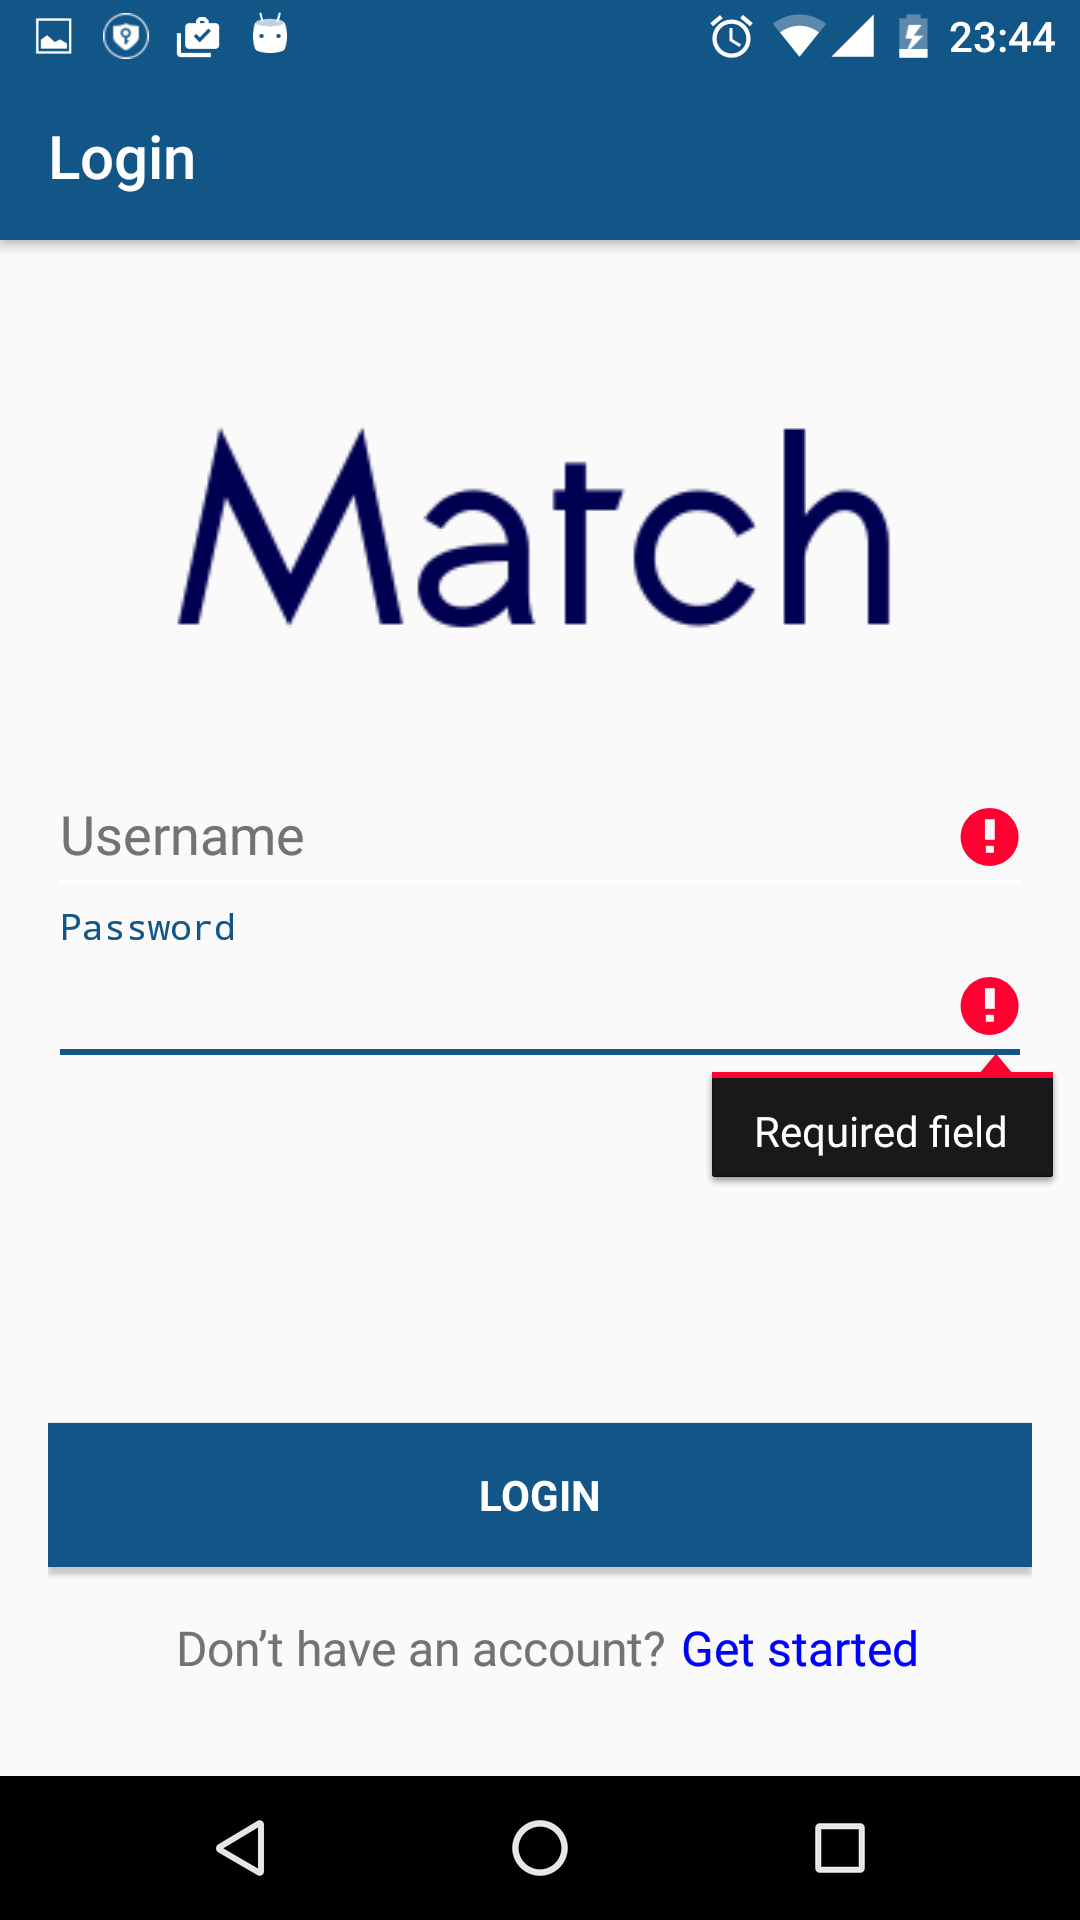
\includegraphics{login_failed.png}
\begin{itemize}
\item {} 
Si no posee un usuario debera crear uno haciendo tap en el texto “Get started” de la pantalla de login. Se lo redireccionara a la pantalla de registro.

\end{itemize}

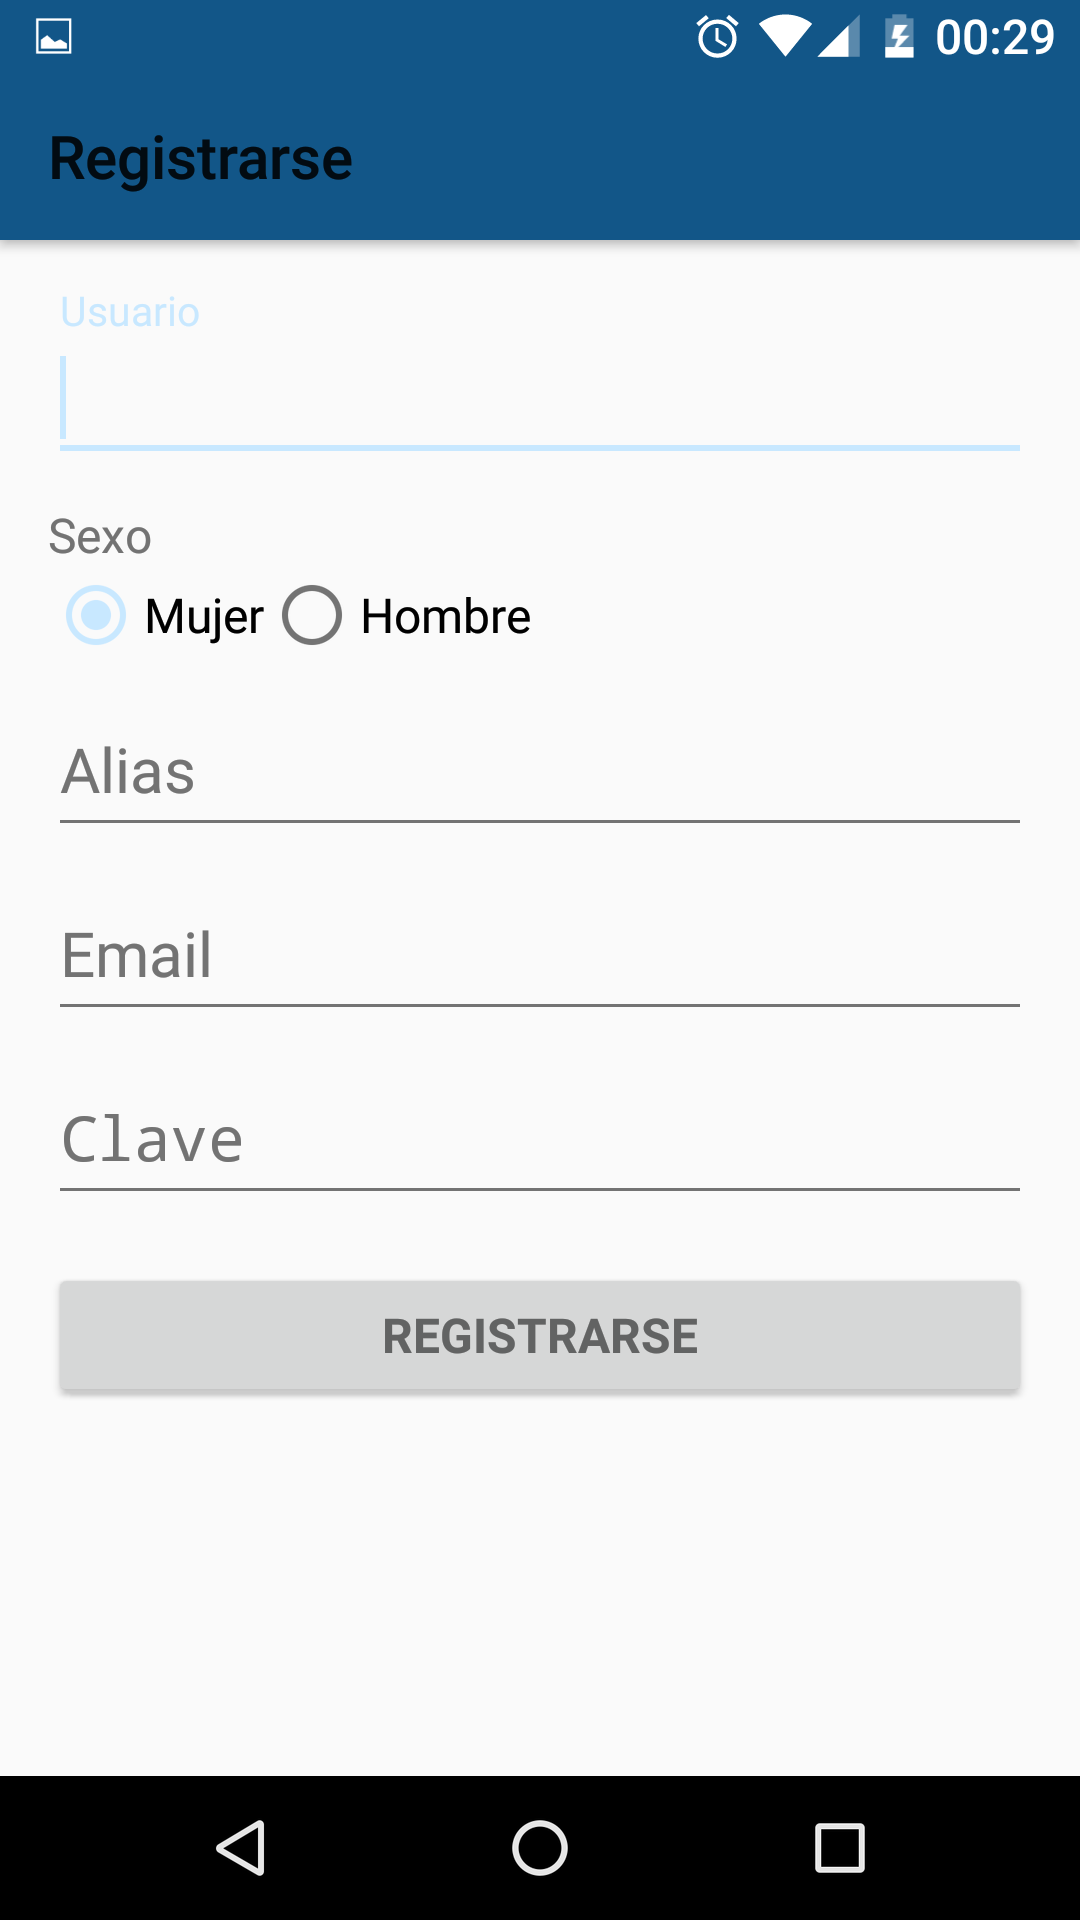
\includegraphics{registro.png}
\begin{itemize}
\item {} 
Llene los datos requeridos para crear el usuario, para elegir los intereses haga click en pick interests.

\end{itemize}

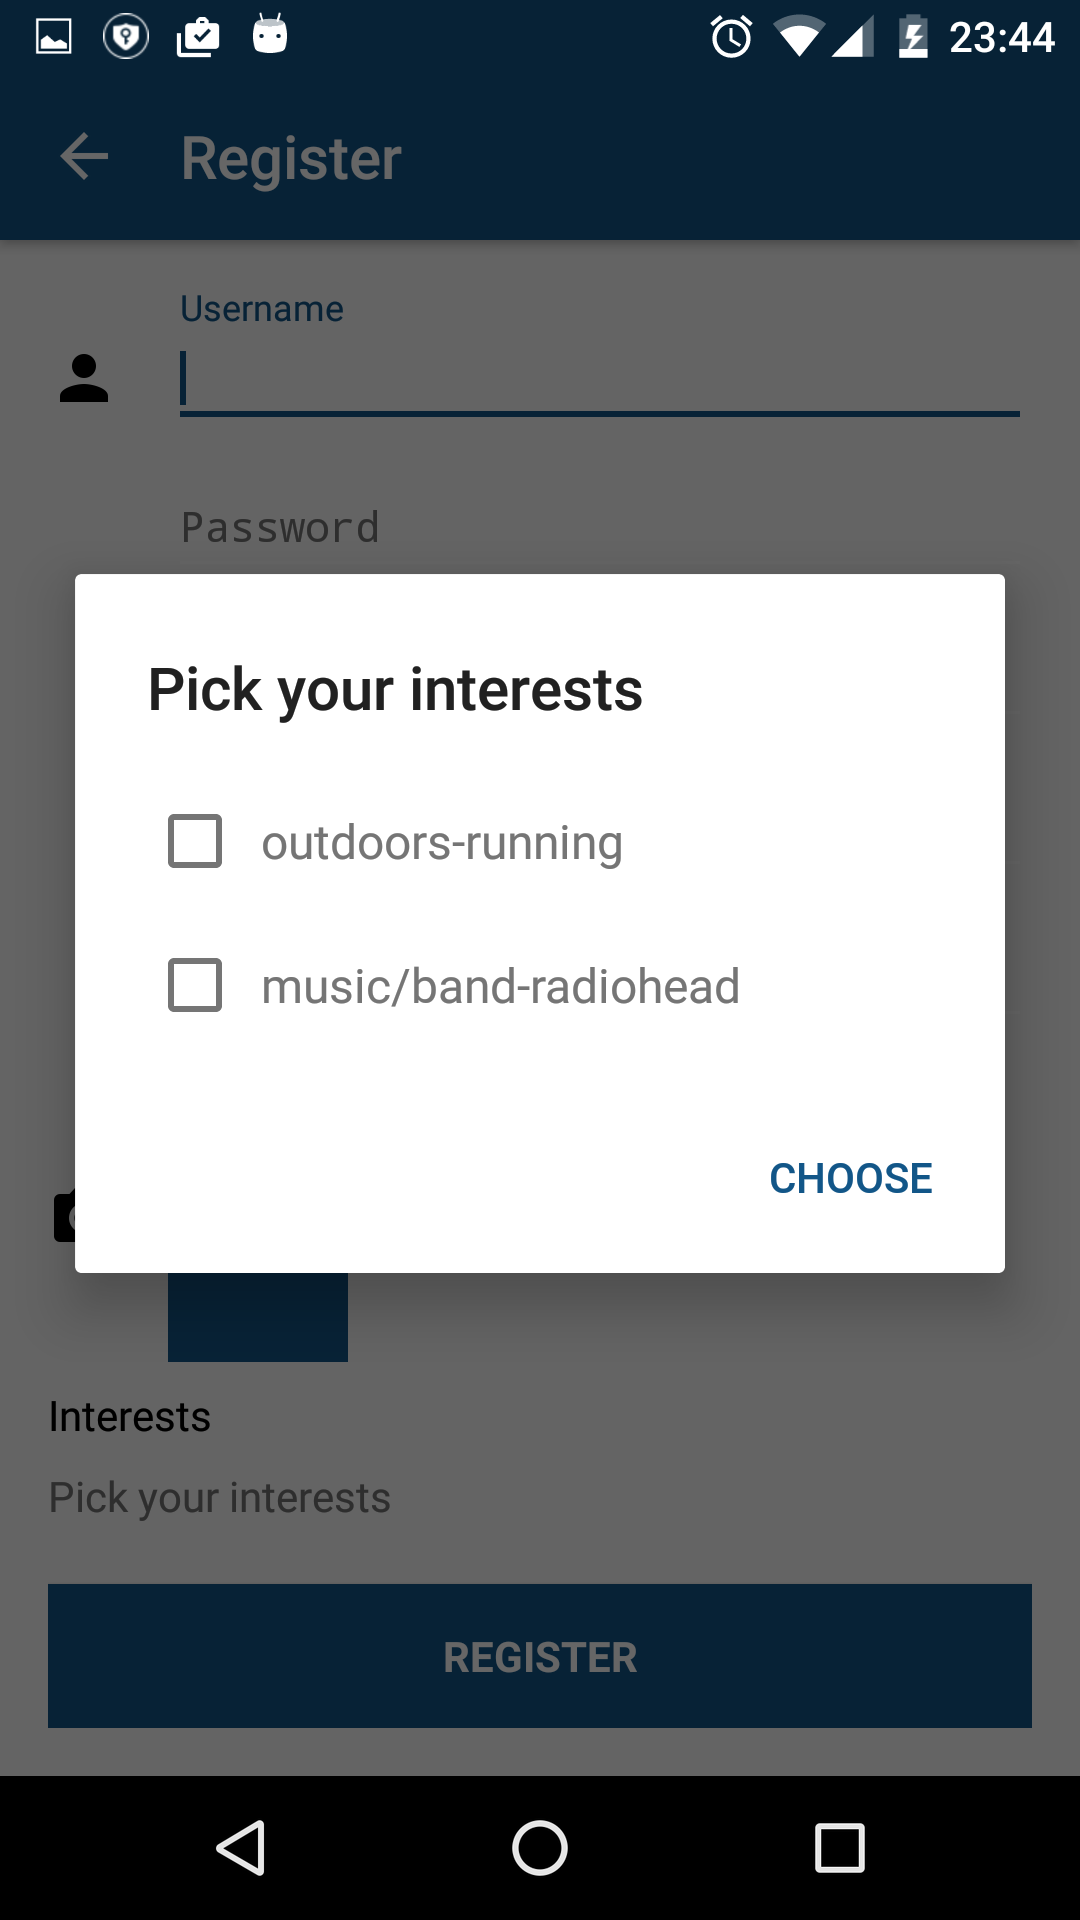
\includegraphics{interests.png}
\begin{itemize}
\item {} 
Haga tap en Register para crear el nuevo usuario.

\item {} 
Si los datos son correctos se lo redireccionara a la pantalla de login para que pueda ingresar a la aplicacion.

\item {} 
Si los datos son erroneos aparecera un mensaje de error y debera reintentar el registro.

\end{itemize}

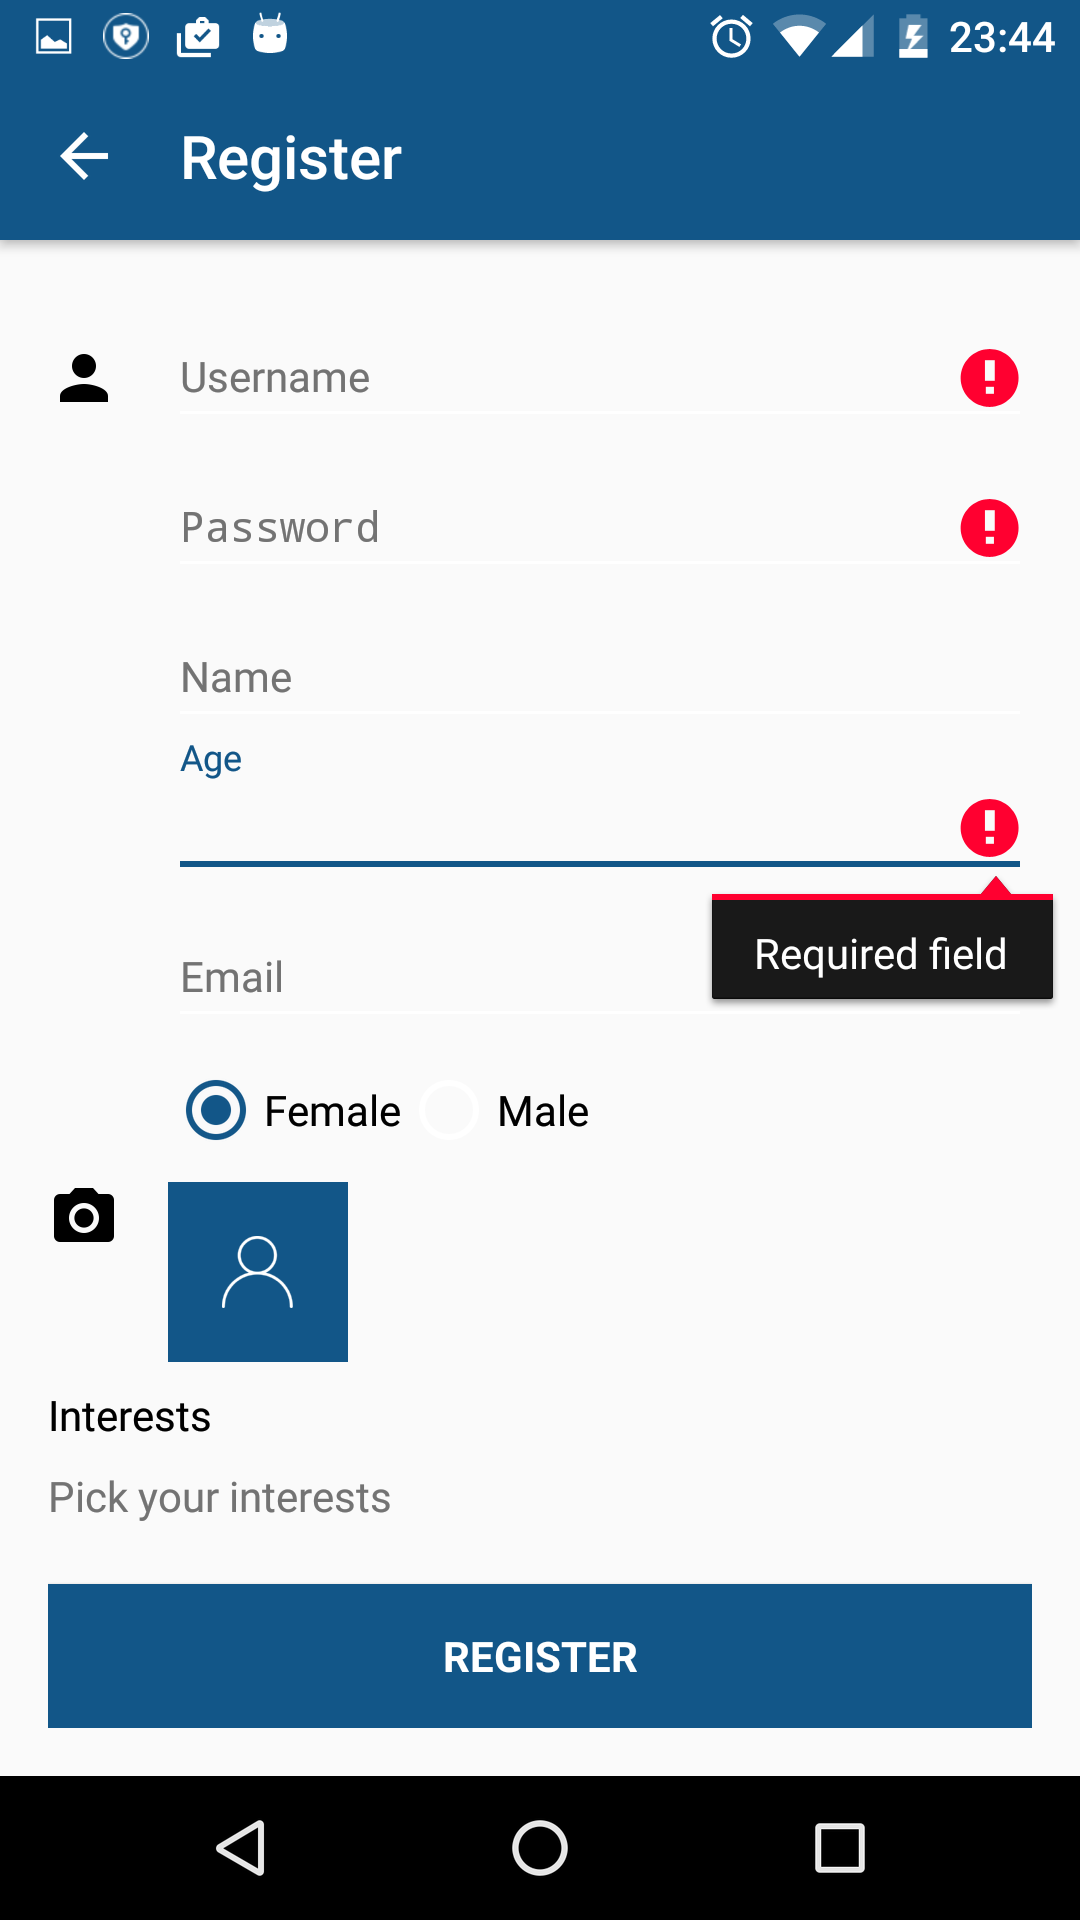
\includegraphics{registro_failed.png}
\begin{itemize}
\item {} 
Al loguearse se lo redireccionara a la pantalla de busqueda de matches

\end{itemize}

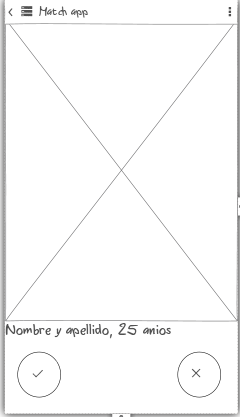
\includegraphics{match.png}
\begin{itemize}
\item {} 
Podra navegar entre los candidatos haciendo swipe en la pantalla, podra moverse a la derecha o a la izquierda.

\item {} 
Podra darle un like o un dislike al candidato haciendo click en los botones flotantes.

\item {} 
Si hay match de ambos lados se abrira la pantalla de chat y podran mandarse mensajes entre ambos usuarios.

\end{itemize}

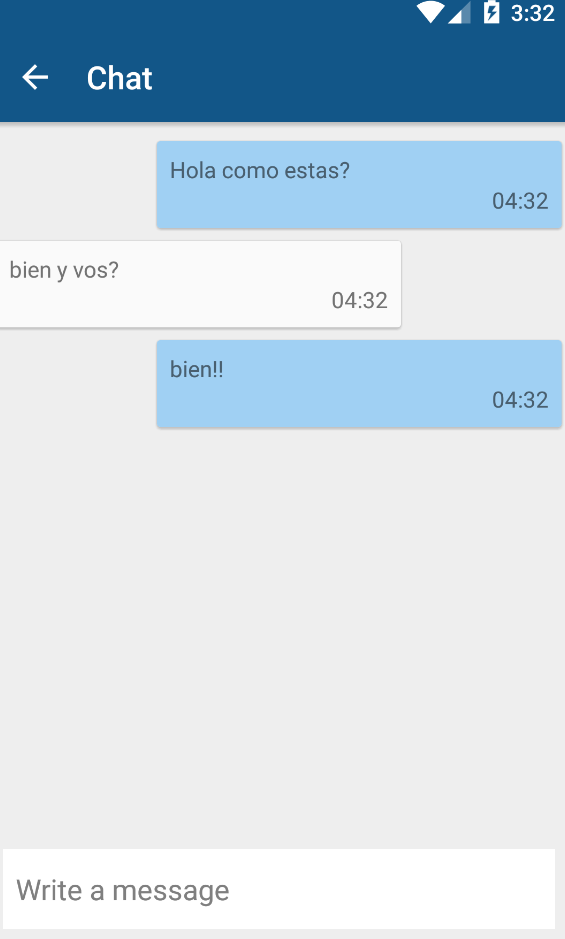
\includegraphics{chat.png}
\begin{itemize}
\item {} 
Podra ver sus matches disponibles desde la pantalla de matches disponibles, ingresando desde el menu lateral.

\end{itemize}

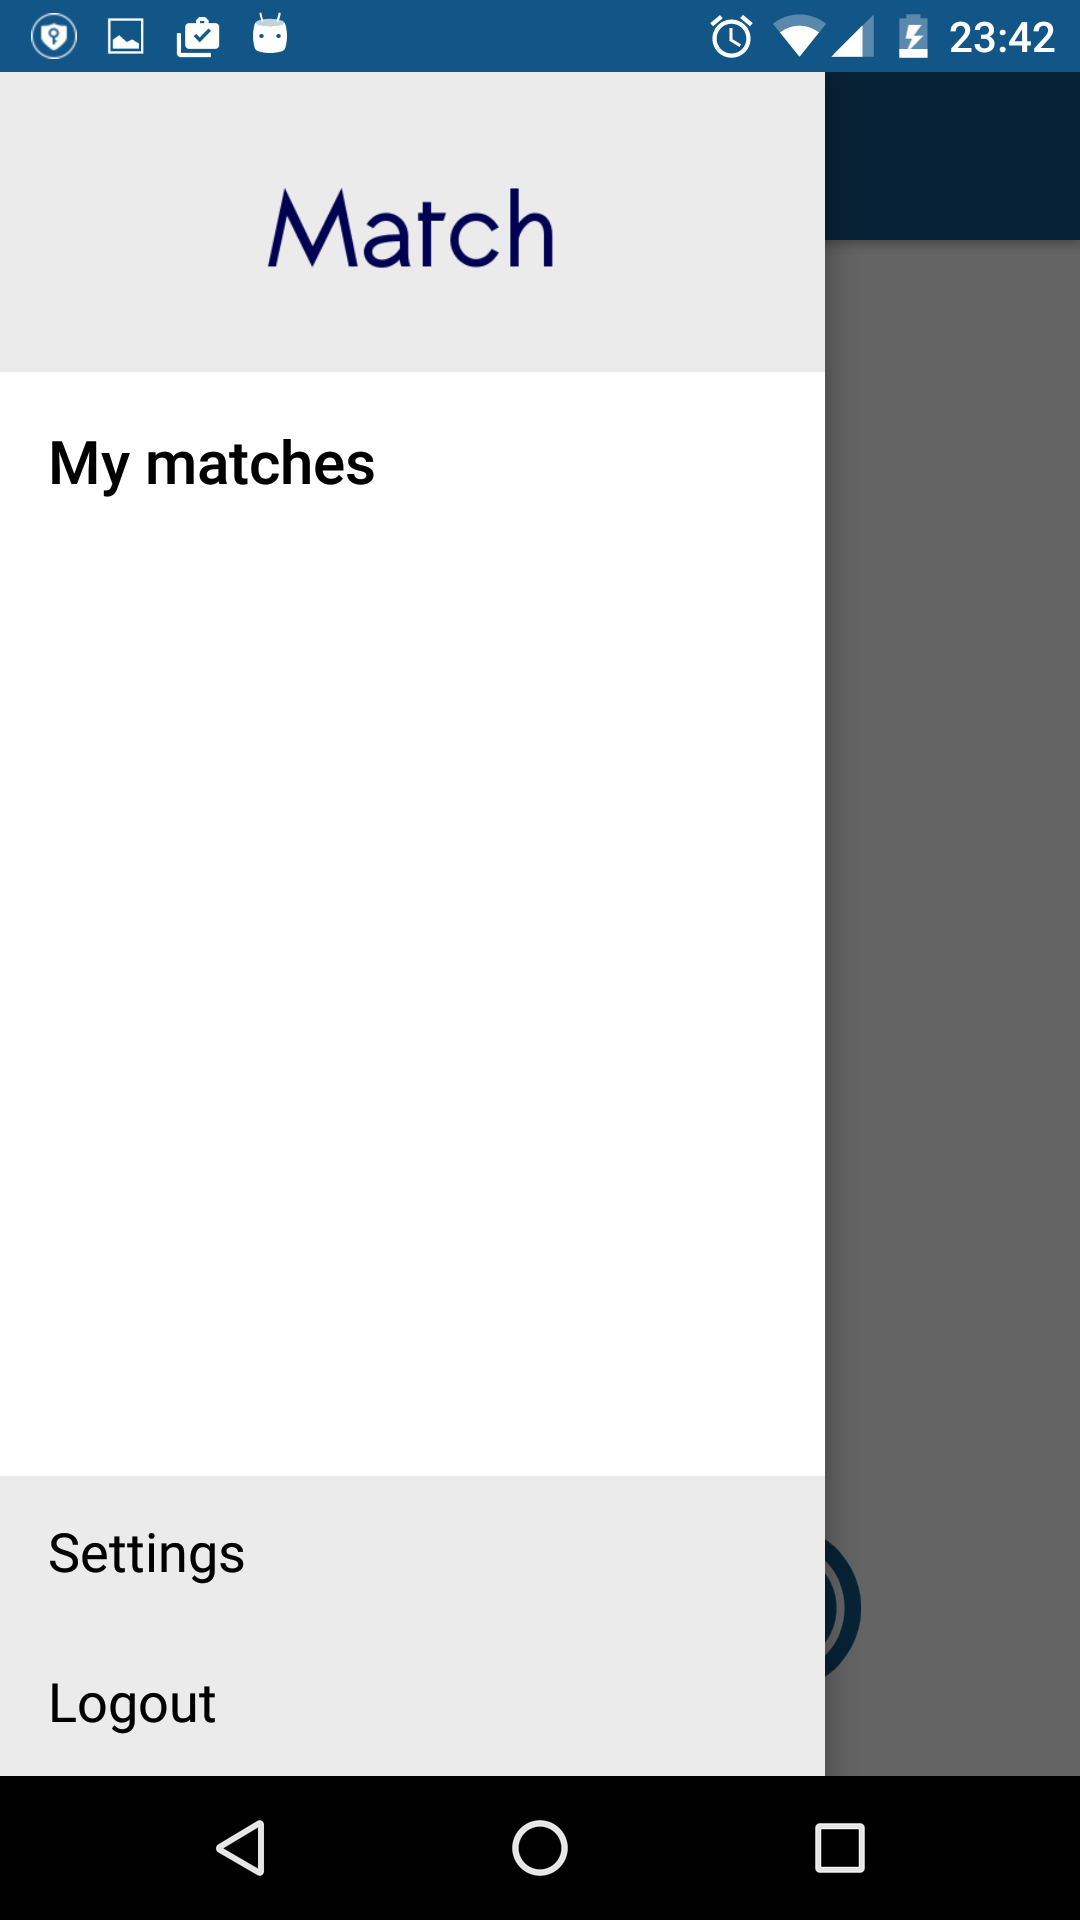
\includegraphics{sidebar.png}
\begin{itemize}
\item {} 
Podra cambiar sus intereses desde su perfil, ingresando desde el menu lateral.

\end{itemize}

\includegraphics{Screenshots/interestsChange.png}


\section{Shared Server}
\label{manuals:shared-server}\begin{itemize}
\item {} 
Para comenzar a utilizar el Shared Server, debe redirigirse con su navegador al sitio \href{https://tallerdeprogramacionii-1c2016.herokuapp.com/}{https://tallerdeprogramacionii-1c2016.herokuapp.com/}. Una vez ingresado allí, observará la portada inicial del sitio como la que se muestra a continuación:

\end{itemize}

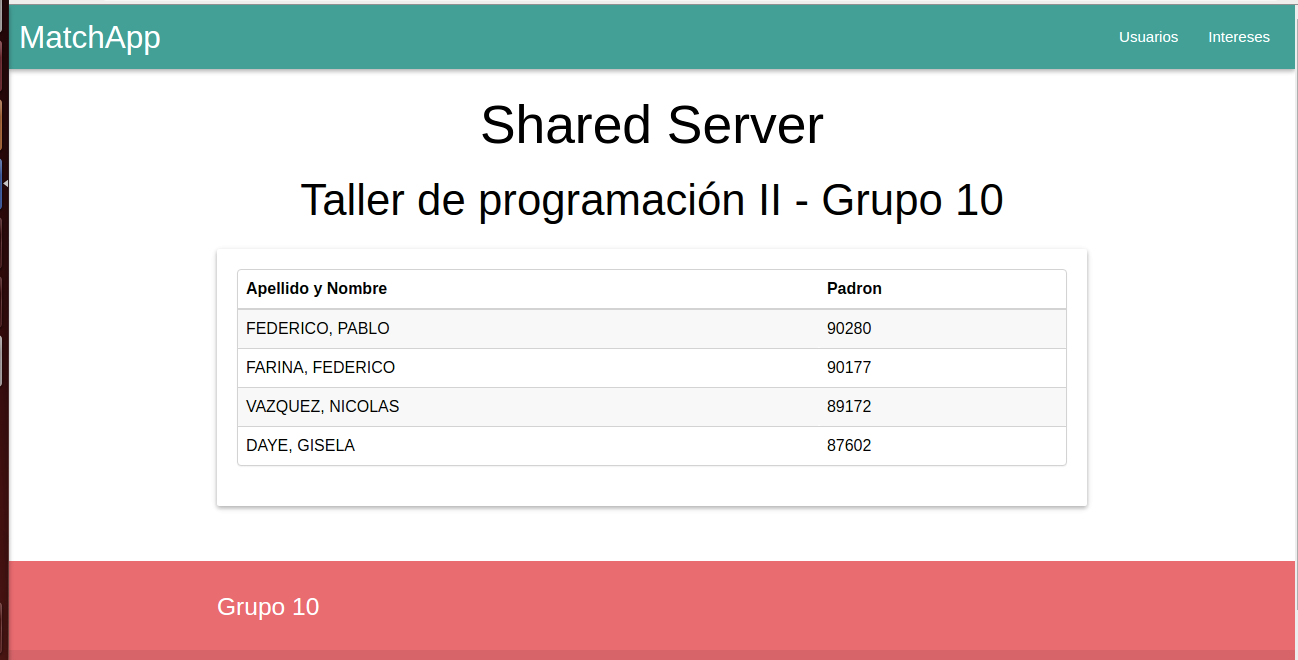
\includegraphics{shared_portada.png}
\begin{itemize}
\item {} 
Para dar de alta un usuario haga click en “Alta usuario”. Se lo redireccionara a la pantalla para dar de alta al usuario

\end{itemize}

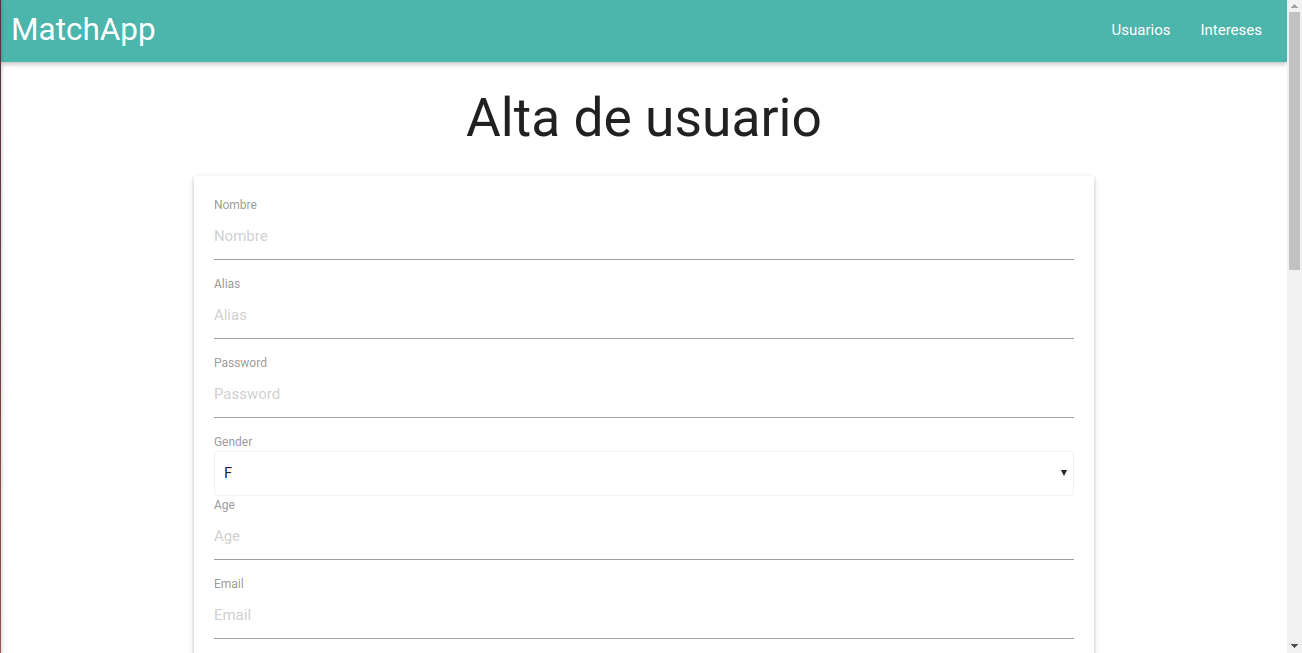
\includegraphics{shared_altaUsuario.png}
\begin{itemize}
\item {} 
Al ingresar, se le mostrará una advertencia para poder activar la Geolocalización a fin de saber sus posiciones geográficas

\end{itemize}

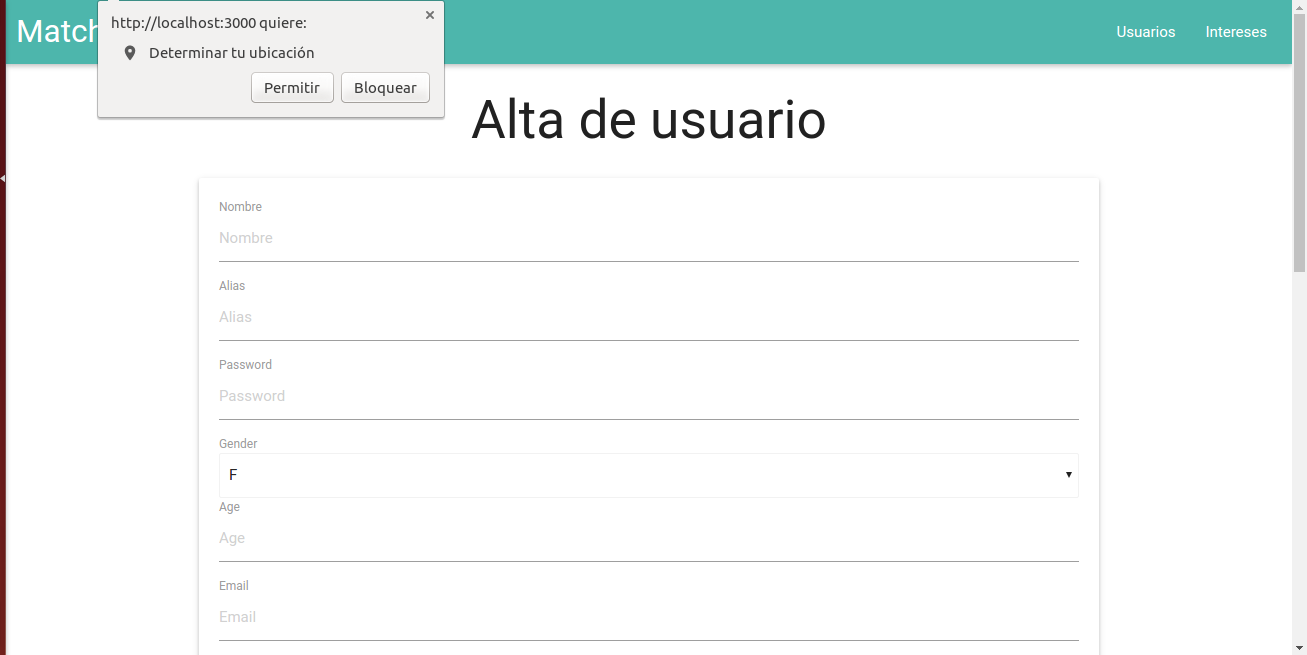
\includegraphics{shared_localizacion.png}
\begin{itemize}
\item {} 
Al aceptar, se mostrará en la parte inferior del formulario de carga de usuario, su localización

\end{itemize}

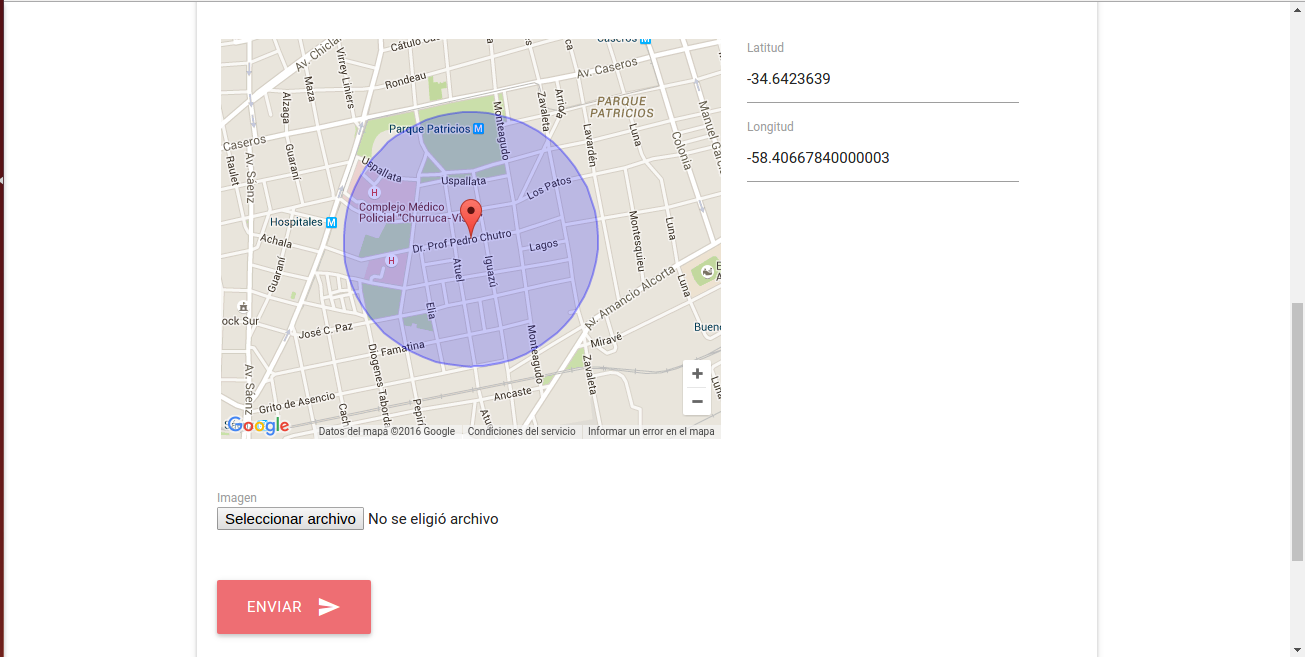
\includegraphics{shared_localizacion2.png}
\begin{itemize}
\item {} 
Ingrese lo datos requeridos y haga click en el boton “Enviar” para agregar un usuario a Match App.

\item {} 
Para ver los usuarios registrados seleccione la opción ``Usuarios'' desde la portada del sitio. Se redireccionara a la pantalla de listado de usuarios

\end{itemize}

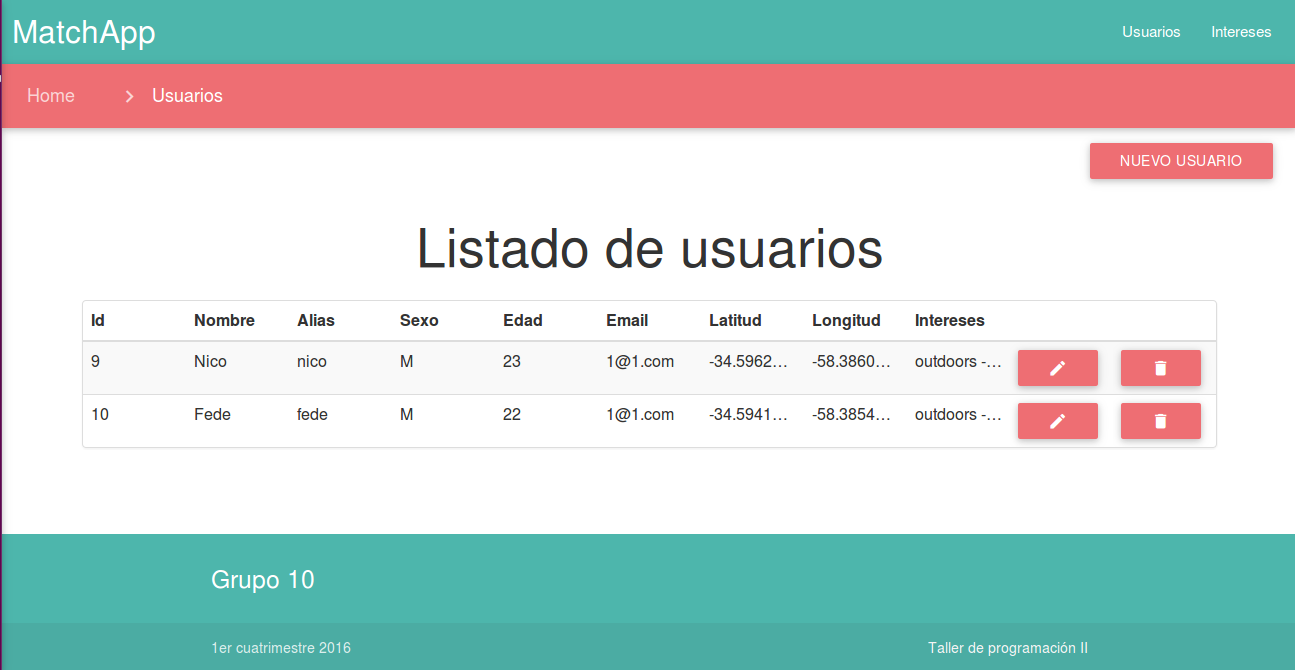
\includegraphics{shared_listadoUsuarios.png}
\begin{itemize}
\item {} 
Cada usuario se puede borrar, eliminandolo completamente de la aplicación. Para ello solo debe hacer click en el icono de borrado al lado de cada usuario. Además, se podran editar las propiedades de cada usuario, haciendo click en el icono en forma de lapiz al lado del usuario. Si se selecciona la edición de un usuario, la aplicación lo redireccionará a una nueva pantalla, como la que se muestra a continuación

\end{itemize}

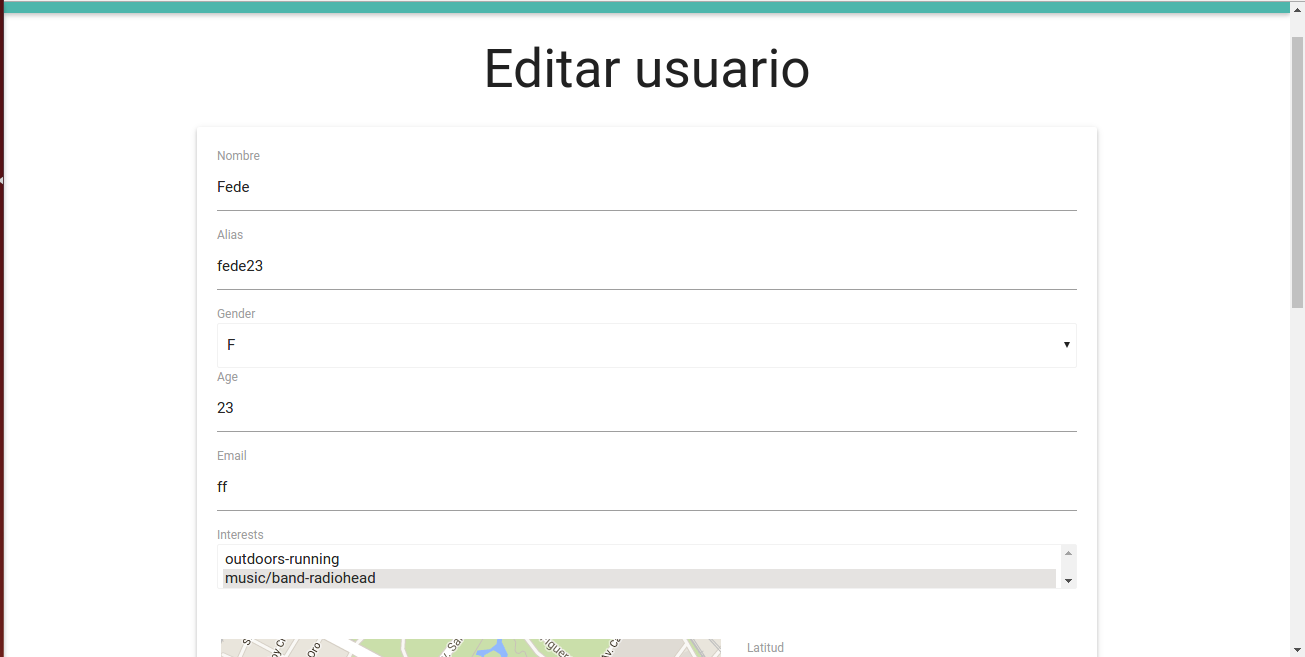
\includegraphics{shared_editUsuarios.png}
\begin{itemize}
\item {} 
La pantalla le mostrará los datos cargados por el usuario. Una vez finalizada la edición, click en ``Enviar'' para guardar los cambios

\item {} 
Además, se podran agregar y borrar los intereses permitidos en la aplicación. Para ingresar, dirigirse a la portada y seleccionar ``Intereses'' en el margen superior derecho. Esto lo llevará a la pantalla con el listado de intereses actuales

\end{itemize}

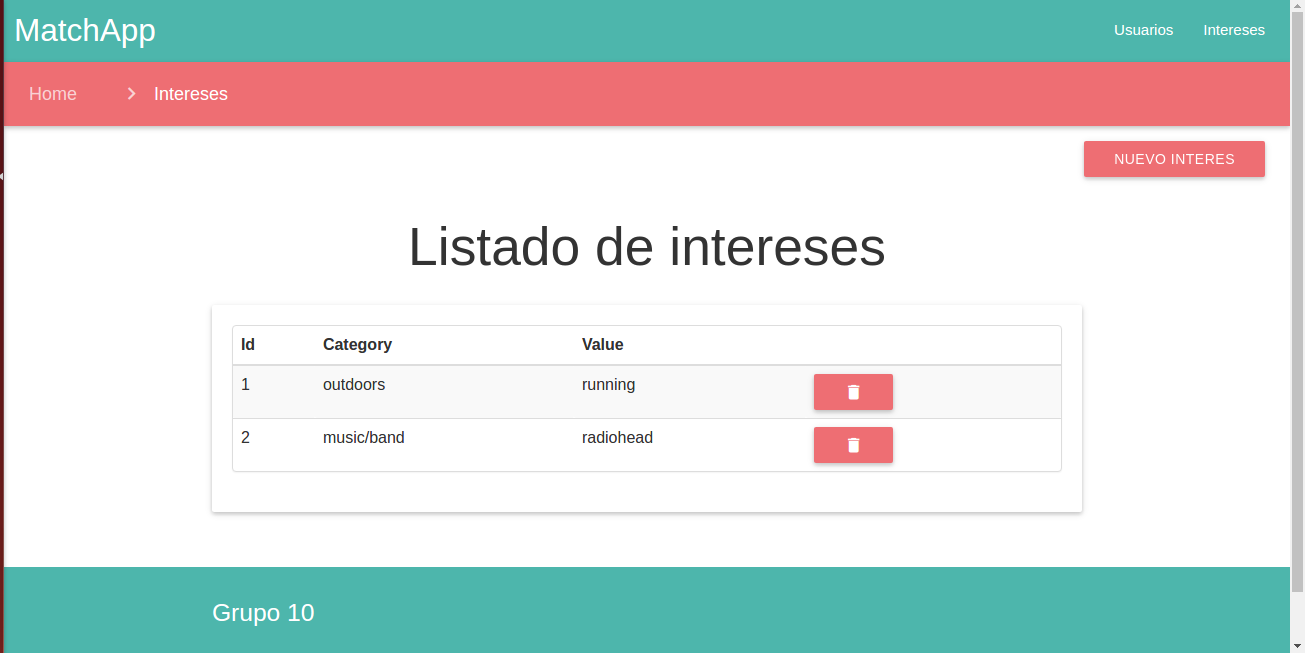
\includegraphics{shared_listadoIntereses.png}
\begin{itemize}
\item {} 
Para dar de alta una nueva intereses, debe hacer click en el botón de ``Alta interes''.

\end{itemize}

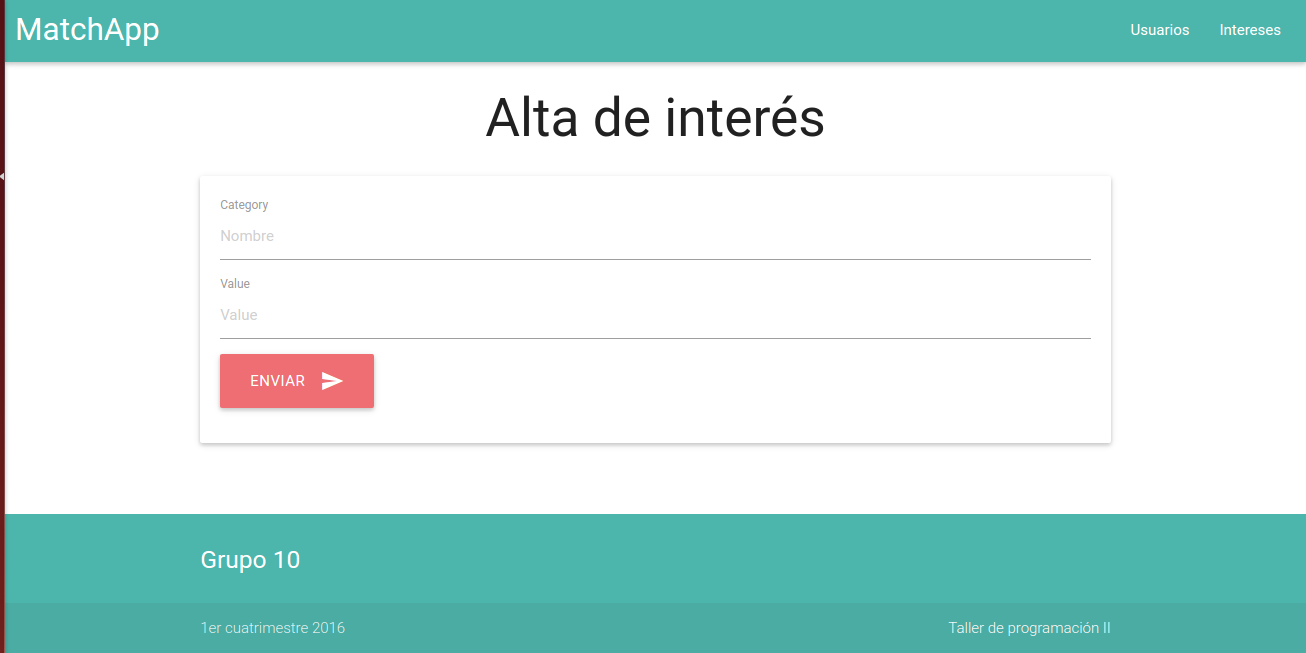
\includegraphics{shared_altaInteres.png}
\begin{itemize}
\item {} 
Luego de completar los campos, hacer click en Enviar para dar de alta el nuevo interés.

\item {} 
Se podra borrar un interes haciendo click en el botón que se encuentra al lado de cada interés.

\end{itemize}


\chapter{Indices y tablas}
\label{index:indices-y-tablas}\begin{itemize}
\item {} 
\emph{genindex}

\item {} 
\emph{modindex}

\item {} 
\emph{search}

\end{itemize}



\renewcommand{\indexname}{Index}
\printindex
\end{document}
